\documentclass[12pt, titlepage]{article}

\usepackage{booktabs}
\usepackage{tabularx}
\usepackage{hyperref}
\usepackage{graphicx}
\usepackage{float}
\hypersetup{
    colorlinks,
    citecolor=blue,
    filecolor=black,
    linkcolor=red,
    urlcolor=blue
}
\usepackage[round]{natbib}

%% Comments

\usepackage{color}

\newif\ifcomments\commentstrue %displays comments
%\newif\ifcomments\commentsfalse %so that comments do not display

\ifcomments
\newcommand{\authornote}[3]{\textcolor{#1}{[#3 ---#2]}}
\newcommand{\todo}[1]{\textcolor{red}{[TODO: #1]}}
\else
\newcommand{\authornote}[3]{}
\newcommand{\todo}[1]{}
\fi

\newcommand{\wss}[1]{\authornote{blue}{SS}{#1}} 
\newcommand{\plt}[1]{\authornote{magenta}{TPLT}{#1}} %For explanation of the template
\newcommand{\an}[1]{\authornote{cyan}{Author}{#1}}

%% Common Parts

\newcommand{\progname}{Housemates} % PUT YOUR PROGRAM NAME HERE
\newcommand{\authname}{Team \#9, Housemates
\\ Justin Dang - dangj15 
\\ Harris Hamid - hamidh1
\\ Fady Morcos - morcof2 
\\ Rizwan Ahsan - ahsanm7
\\ Sheikh Afsar - afsars} % AUTHOR NAMES                  

\usepackage{hyperref}
    \hypersetup{colorlinks=true, linkcolor=blue, citecolor=blue, filecolor=blue,
                urlcolor=blue, unicode=false}
    \urlstyle{same}
                                


\begin{document}

\title{Verification and Validation Plan for \progname{}} 
\author{\authname}
\date{March 6, 2024}
	
\maketitle

\pagenumbering{roman}

\section*{Revision History}

\begin{tabularx}{\textwidth}{p{3cm}p{2cm}X}
\toprule {\bf Date} & {\bf Version} & {\bf Notes}\\
\midrule
Nov 3 2023 & 0 & Revision 0\\
Mar 6 2024 & 1 & Update with Unit Testing\\
\bottomrule
\end{tabularx}

% ~\\
% \wss{The intention of the VnV plan is to increase confidence in the software.
% However, this does not mean listing every verification and validation technique
% that has ever been devised.  The VnV plan should also be a \textbf{feasible}
% plan. Execution of the plan should be possible with the time and team available.
% If the full plan cannot be completed during the time available, it can either be
% modified to ``fake it'', or a better solution is to add a section describing
% what work has been completed and what work is still planned for the future.}

% \wss{The VnV plan is typically started after the requirements stage, but before
% the design stage.  This means that the sections related to unit testing cannot
% initially be completed.  The sections will be filled in after the design stage
% is complete.  the final version of the VnV plan should have all sections filled
% in.}

\newpage

\tableofcontents

% \listoftables
% \wss{Remove this section if it isn't needed}

% \listoffigures
% \wss{Remove this section if it isn't needed}

\newpage

% \section{Symbols, Abbreviations, and Acronyms}

% \renewcommand{\arraystretch}{1.2}
% \begin{tabular}{l l} 
%   \toprule		
%   \textbf{symbol} & \textbf{description}\\
%   \midrule 
%   T & Test\\
%   \bottomrule
% \end{tabular}\\

% \wss{symbols, abbreviations, or acronyms --- you can simply reference the SRS
%   \citep{SRS} tables, if appropriate}

% \wss{Remove this section if it isn't needed}

\newpage

\pagenumbering{arabic}

% This document ... \wss{provide an introductory blurb and roadmap of the
%   Verification and Validation plan}

\section{General Information}

\subsection{Summary}

 Housemates is an application that will allow its users to communicate with their housemates more effectively. The Housemates application will have a cost management system to split costs amongst housemates, a chore management system to delegate tasks amongst housemates, and a scheduling system to allow housemates to schedule events.

% \wss{Say what software is being tested.  Give its name and a brief overview of
%   its general functions.}

\subsection{Objectives}

The objective of this verification and validation plan is to
\begin{enumerate}
    \item Ensure that the requirements listed in the SRS for the Housemates application are correct.
    \item Ensure that the design of the Housemates application satisfies the requirements listed in the SRS.
    \item Ensure the usability of the Housemates application for its prospective users.
\end{enumerate}

% \wss{State what is intended to be accomplished.  The objective will be around
%   the qualities that are most important for your project.  You might have
%   something like: ``build confidence in the software correctness,''
%   ``demonstrate adequate usability.'' etc.  You won't list all of the qualities,
%   just those that are most important.}

% \wss{You should also list the objectives that are out of scope.  You don't have 
% the resources to do everything, so what will you be leaving out.  For instance, 
% if you are not going to verify the quality of usability, state this.  It is also 
% worthwhile to justify why the objectives are left out.}

% \wss{The objectives are important because they highlight that you are aware of 
% limitations in your resources for verification and validation.  You can't do everything, 
% so what are you going to prioritize?  As an example, if your system depends on an 
% external library, you can explicitly state that you will assume that external library 
% has already been verified by its implementation team.}

\subsection{Relevant Documentation}

% \wss{Reference relevant documentation.  This will definitely include your SRS
%   and your other project documents (design documents, like MG, MIS, etc).  You
%   can include these even before they are written, since by the time the project
%   is done, they will be written.}

\begin{itemize}
    \item \href{https://github.com/DangJustin/CapstoneProject/blob/main/docs/DevelopmentPlan/DevelopmentPlan.pdf}{Development Plan}: The development plan contains the tools planned to be used in the development of the application along with the overall schedule for this project. These items will be referenced to in this VnV plan.  
    \item \href{https://github.com/DangJustin/CapstoneProject/blob/main/docs/SRS-Volere/SRS.pdf}{SRS}: The software requirements specification contains the functional and non-functional requirements of the Housemates application. These requirements will be tested for in the VnV plan under system testing. 
    \item \href{https://github.com/DangJustin/CapstoneProject/blob/main/docs/HazardAnalysis/HazardAnalysis.pdf}{Hazard Analysis}: The hazard analysis document contains the hazards associated with the application. These hazards will need to be tested for in the VnV plan in order to be sure that they are mitigated.
    \item \href{https://github.com/DangJustin/CapstoneProject/tree/main/docs/Design}{Design}: The design document will contain the underlying design of the Housemates application. The elements of this design will be tested in the unit testing section of this VnV plan.
    \item \href{https://github.com/DangJustin/CapstoneProject/blob/main/docs/VnVReport/VnVReport.pdf}{VnV Repor}t: The VnV report will document the results of the VnV plan used in this document.
\end{itemize}


% \citet{SRS}

% \wss{Don't just list the other documents.  You should explain why they are relevant and 
% how they relate to your VnV efforts.}

\section{Plan}

This section contains the different verification and validation plans that will be used throughout the project along with the team responsible for executing them.  

% \wss{Introduce this section.   You can provide a roadmap of the sections to
%   come.}

\subsection{Verification and Validation Team}

\begin{itemize}
    \item Justin Dang: Will focus on task management system and performance testing.
    \item Harris Hamid: Will focus on bill management system and usability testing.
    \item Fady Marcos: Will focus on Account system, scheduling system as a part of functional testing
    \item Rizwan Ahsan: Will focus on task management system and usability testing. 
    \item Sheikh Afsar: Will focus on bill management system and usability testing.
\end{itemize}


% \wss{Your teammates.  Maybe your supervisor.
%   You should do more than list names.  You should say what each person's role is
%   for the project's verification.  A table is a good way to summarize this information.}

\subsection{SRS Verification Plan}

\begin{itemize}
    \item Classmates will review the SRS documentation.
    \item A TA for SFWRENG 4G06 will review the SRS documentation.
    \item The SRS checklist listed in the Checklists folder will be used by the verification and validation team to review the SRS documentation.
    \item A focus group with potential users of the application will be shown a wire-frame version of the Housemates to see if fits user needs.
\end{itemize}

% \wss{List any approaches you intend to use for SRS verification.  This may include
%   ad hoc feedback from reviewers, like your classmates, or you may plan for 
%   something more rigorous/systematic.}

% \wss{Maybe create an SRS checklist?}

\subsection{Design Verification Plan}


\begin{itemize}
    \item Classmates will review the Design documentation.
    \item A TA for SFWRENG 4G06 will review the Design documentation.
    \item The Design checklists in the Checklists folder will be used by the verification and validation team to review the Design documentation.
\end{itemize}

% \wss{Plans for design verification}

% \wss{The review will include reviews by your classmates}

% \wss{Create a checklists?}

\subsection{Verification and Validation Plan Verification Plan}

\begin{itemize}
    \item Classmates will review the VnV documentation.
    \item A TA for SFWRENG 4G06 will review the VnV documentation.
    \item The VnV checklist listed in the Checklists folder will be used by the verification and validation team to review the VnV documentation.
    \item The tests in the VnV plan will be executed and the results will be documented in the VnV report.
\end{itemize}



% \wss{The verification and validation plan is an artifact that should also be
% verified.  Techniques for this include review and mutation testing.}

% \wss{The review will include reviews by your classmates}

% \wss{Create a checklists?}

\subsection{Implementation Verification Plan}

Verification of the implementation will be conducted through performing the system tests described in the VnV plan.

% After the completion of the Housemates application a code inspection and walkthrough will be conducted on the source code of the application. This will be used to identify any potential errors in the source code that prevent the application from satisfying its requirements.

% \wss{You should at least point to the tests listed in this document and the unit
%   testing plan.}

% \wss{In this section you would also give any details of any plans for static
%   verification of the implementation.  Potential techniques include code
%   walkthroughs, code inspection, static analyzers, etc.}

\subsection{Automated Testing and Verification Tools}

Automatic testing of the document will be done through the jest.

% \wss{What tools are you using for automated testing.  Likely a unit testing
%   framework and maybe a profiling tool, like ValGrind.  Other possible tools
%   include a static analyzer, make, continuous integration tools, test coverage
%   tools, etc.  Explain your plans for summarizing code coverage metrics.
%   Linters are another important class of tools.  For the programming language
%   you select, you should look at the available linters.  There may also be tools
%   that verify that coding standards have been respected, like flake9 for
%   Python.}

% \wss{If you have already done this in the development plan, you can point to
% that document.}

% \wss{The details of this section will likely evolve as you get closer to the
%   implementation.}

\subsection{Software Validation Plan}

We plan to conduct user testing on a focus group of potential users of the Housemates application after the Revision 0 version is complete. The user testing will be using the usability survey questions as described in the appendix.

% \wss{If there is any external data that can be used for validation, you should
%   point to it here.  If there are no plans for validation, you should state that
%   here.}

% \wss{You might want to use review sessions with the stakeholder to check that
% the requirements document captures the right requirements.  Maybe task based
% inspection?}

% \wss{For those capstone teams with an external supervisor, the Rev 0 demo should 
% be used as an opportunity to validate the requirements.  You should plan on 
% demonstrating your project to your supervisor shortly after the scheduled Rev 0 demo.  
% The feedback from your supervisor will be very useful for improving your project.}

% \wss{For teams without an external supervisor, user testing can serve the same purpose 
% as a Rev 0 demo for the supervisor.}

% \wss{This section might reference back to the SRS verification section.}

\section{System Test Description}
	
\subsection{Tests for Functional Requirements}

This section contains the tests for the functional requirements. The subsections in this section are based off the SRS and cover the different features of the Housemates application. The fit criterion for each functional requirement of the SRS are used here to help create tests for those functional requirements

% \wss{Subsets of the tests may be in related, so this section is divided into
%   different areas.  If there are no identifiable subsets for the tests, this
%   level of document structure can be removed.}

% \wss{Include a blurb here to explain why the subsections below
%   cover the requirements.  References to the SRS would be good here.}

\subsubsection{Task Management System}

This subsection covers the tests for the task management system of the Housemates application. The task management system of the housemates application will allow users to split and delegate common household tasks to their housemates.

% \wss{It would be nice to have a blurb here to explain why the subsections below
%   cover the requirements.  References to the SRS would be good here.  If a section
%   covers tests for input constraints, you should reference the data constraints
%   table in the SRS.}

\begin{enumerate}

\item{test-TM1-1\\}

Description: Verify navigation to Task Management page via tasks icon.
					
Initial State: Housemates app is open.
					
Input: Tap on the tasks icon.
					
Output: User is taken to the Task Management page.

Test Case Derivation: This is to be able to navigate to the task management page of the app instead of utilizing one of the other features.
					
How test will be performed: 
Open the Housemates app.
Tap on the tasks icon.
Verify that the Task Management page is displayed.
					
\item{test-TM2-1\\}

Control: Manual

Description: Verify that the Task Management page displays a list of tasks with user's chores highlighted.
					
Initial State: Task Management page is open.
					
Input: None.
					
Output: User can clearly identify their assigned tasks.

Test Case Derivation: This is to be able to clearly view the tasks which the user must complete.

How test will be performed: 
Open the Task Management page.
Verify that a list of tasks is displayed, with user's chores highlighted.

\item{test-TM3-1\\}

Control: Manual

Description: Verify creation of a new task.
					
Initial State: Task Management page is open.
					
Input: Task Name: "Clean the Living Room"
Due Date: 2024-4-05
					
Output: New task "Clean the Living Room" is added to the list of tasks.

Test Case Derivation: Users need to be able to add new chores/tasks as needed.

How test will be performed: 
Open the Task Management page.
Click on "Create New Task" button.
Fill out the task creation form with the provided input.
Click "Create" button.
Verify that the new task appears in the list of tasks.


\item{test-TM4-1\\}

Control: Manual

Description: Verify assigning a task to a roommate.
					
Initial State: Task Management page is open.
					
Input: Task Name: "Take out the garbage".
Due Date: 2024-4-05
Roommate Assignment: Fardeen Afsar.
					
Output: Task is assigned to Fardeen, Fardeen can see.

Test Case Derivation: This feature enables users to divide tasks among roommates.

How test will be performed: 
Open the Task Management page.
Create a task.
Choose roommate "Fardeen" from the list of roommates.
Login as Fardeen
Verify that the task is now assigned to Fardeen and Fardeen can see task.

\item{test-TM5-1\\}

Control: Manual

Description: Verify marking a task as completed.
					
Initial State: Task Management page is open with at least one task.
					
Input: Task Name: Select a task from the list.
Mark task as completed.
					
Output: Task is marked as completed and status is updated.

Test Case Derivation: Users need to be allowed to track the progress of tasks and mark them as completed when they are done.

How test will be performed: 
Open the Task Management page.
Select a task from the list.
Mark the task as completed.
Verify that the task is now marked as completed on the Task Management page.



\end{enumerate}

\subsubsection{Bill Management System}

This subsection covers the tests for the bill management system of the Housemates application. The bill management system of the housemates application will allow users to split bills with their housemates who incur a specific expense.

\begin{enumerate}

\item{test-BM1-1/2-1\\}

This test checks whether a user is able to create a new bill and assign housemates to it

Control: Manual
					
Initial State: The bill management system is active and ready to handle events the user provides.
					
Input: Total amount incurred and users who to split among.
					
Output: A bill is generated with provided total amount being split evenly among housemates.

Test Case Derivation: The system expects a positive value in a specified format according to the chosen currency which is provided in the input the chosen users to share the expense with thus accepted by the system.
					
How test will be performed: A tester will be provided instructions to follow with a valid bill amount and associated housemates. The tester will then determine by cross-checking whether the result provided by the system matches with the actual result in the instructions.
					
\item{test-BM3-1\\}

This test ensures whether a user (bill issuer) is able to modify an already existing bill

Control: Manual
					
Initial State: The bill management system is active and ready to handle events the user provides.
					
Input: User selects to edit any past expense, alters previously inputted information as deemed fit and may change the users by adding or removing users. 
					
Output: A new bill is generated with provided total amount being split evenly among housemates Note: this alteration will not change the date on which this expense was incurred.

Test Case Derivation: The system expects a positive value in a specified format according to the chosen currency which is provided in the input and the chosen users to share the expense with thus accepted by the system.

How test will be performed: A tester will be provided instructions to follow with a valid bill amount and associated housemates. The tester will then determine by cross-checking whether the result provided by the system matches with the actual result in the instructions. 

\item{test-BM4-1\\}

This test checks whether a user is able to categorize a bill (e.g. food, utilities etc) when created. 

Control: Manual
					
Initial State: The bill management system is active and ready to handle events the user provides.
					
Input: Select from a pre-defined set of categories to assign the type of bill and other necessary inputs.
					
Output: A bill is generated with provided total amount being split evenly among housemates along with the nature(type) of the bill.

Test Case Derivation: The system expects the user to choose the type of expense for the bill. This will help the system categorize certain bills together for easier retrieval for user.
					
How test will be performed: A tester will be provided instructions to follow with a valid bill amount and associated housemates and the chosen bill category. The tester will then determine by cross-checking whether the category of the bill matches with the actual category generated by the bill.

\item{test-BM5.1/7.1\\}

This test ensures that previously issued bills can be accessed and can verify the status of expense whether it has been paid or not.

Control: Manual
					
Initial State: The bill management system is active and ready to handle events the user provides.
					
Input: User selects to view any past expense. 
					
Output: A bill is shown with status of each user who incurred the expense of whether they have paid or received the amount.

Test Case Derivation: The system expects to show an updated bill of all the user and what each user owes or is owed.

How test will be performed: A tester will be provided instructions to follow. It will include instructions to first view the bill and observe the current status of what user owes what, then log in as a user associated to that bill and settle the expense. Now check the previous bill again and verify whether bill has been updated.

\item{test-BM6.1\\}

This test ensures that users are able to attach relevant receipts to the bill as an image and view at a later period.

Control: Manual
					
Initial State: The bill management system is active and ready to handle events the user provides.
					
Input: User selects option to add attachment and adds total amount with users who to split among.
					
Output: A bill is shown with the total amount split evenly amongst users and an accessible attachment in form of an image as proof of purchase.

Test Case Derivation: The system expects to show the bill with the original receipt and proof of purchase.

How test will be performed: A tester will be provided instructions to follow. It will include instructions to first create a new bill and provide required information in the fields. The tester will then add an image as an attachment and save the bill. Tester will then access the bill from previous bill section and verify whether attachment can be seen. 

\end{enumerate}

\subsubsection{Scheduling  System}

This subsection covers the tests for the scheduling system of the Housemates application. The scheduling system of the housemates application will allow users to schedule events to coordinate with their housemates.

\begin{enumerate}

\item{test-SS1-1\\}
This test is to ensure users can navigate to the scheduling system page.

Control: Manual
					
Initial State: The app is launched and in the home interface.
					
Input: Tap on the scheduling icon.
					
Output: The scheduling page is displayed to the user.

Test Case Derivation: The expected result in the scheduling page appearing when the scheduling icon is tapped, as described in the requirement SS1.
					
How test will be performed: A tester will open the app in the home interface and tap on the scheduling icon. They will verify that the scheduling page is successfully displayed.


\item{test-SS2-1\\}
This test is to ensure users can create new events and schedule them within the scheduling feature.

Control: Manual
					
Initial State: The user is on the scheduling page
					
Input: The user taps on the button to create new event and fills out the event creation form the necessary description.
					
Output: A new event is listed in the scheduling page.

Test Case Derivation: The system expects to populate the scheduling page with a new event and display it to the user. 

How test will be performed: A tester will navigate to the scheduling page, tap on the button to create new event and input necessary details in the form. They will confirm that the new event appears correctly in the scheduling page.

\item{test-SS3-1\\}
This test is to ensure users can view all the events scheduled by other roommates on their calendar within the scheduling system.

Control: Manual
					
Initial State: The user is on the scheduling page that shows the existing events.
					
Input: User views the calendar within the scheduling system.
					
Output: The user can clearly distinguish between personal events and shared roommate events on the calendar.

Test Case Derivation: Since the system will already be populated with different user's events, the scheduling system should clearly display all events on the calendar.

How test will be performed: A tester will access the scheduling page, view the calendar, and verify that personal events and shared roommate events are clearly distinguishable.

\end{enumerate}

\subsubsection{Account System}

This subsection covers the tests for the account system of the Housemates application. The account system of the housemates application will manage and store user data.

\begin{enumerate}

\item{test-AS1-1\\}

Control: Manual

This test is to ensure a user can create an account.

Initial State: The valid user credentials to be input do not exist in the system yet.
					
Input: User selects create account option, then selects the username field, inputs valid username, then selects password field and inputs valid password.
					
Output: Interface displays that user creation was successful and the credentials are now in the system.

Test Case Derivation: The test case is derived based on the requirement of the housemates application that it must allow users to create an account having entered valid and unique credentials and give the user feedback that creation was successful.
					
How test will be performed: Tester will open app, will press create an account, enter valid credentials and verify that the system allows creation with no issues.
					
\item{test-AS1-2\\}

Control: Manual

This test is to ensure that no two users can exist in the system

Initial State: The valid user already exists in the system.
					
Input: User selects create account option, then selects the username field, inputs the valid username that is already in the system, then selects password field and inputs valid password.
					
Output: The system does not create the profile and informs the user that account creation was not successful that username is already taken.

Test Case Derivation: The test case is derived from the requirements of the housemates app that there should not be two users with the same username.

How test will be performed: Tester will open app, select create an account option and input a username that is already taken and valid password then submit the form.

\item{test-AS1-3\\}

Control: Manual

This test is to ensure that no user profile can be created that does not meet the username and password requirements.

Initial State: The invalid user credentials do not exist in the system.
					
Input: User selects create account option, then selects the username field, inputs all cases of invalid passwords and all cases of invalid usernames that is already in the system, then selects password field and inputs valid password.
					
Output: The system does not create the profile and informs the user of the credential requirements and that creation was not successful due to invalid credentials.

Test Case Derivation: The test case is derived from the requirements of the housemates app which is that user credentials must meet certain requirements.

How test will be performed: Tester will open app, select create an account option and input an invalid username and/or password. Tester will test valid username with invalid password, invalid username with valid password and a case where they are both invalid. Tester will also test all cases of invalid username and all cases of invalid password.

\item{test-AS2\\}

Control: Manual

This test is to ensure that users can login.

Initial State: The  user credentials do exist in the system.
					
Input: User selects login option, then enters user credentials.
					
Output: The system lets the user login.

Test Case Derivation: This is derived based on the requirement that users can have working credentials which they can log into the system with.

How test will be performed: Tester will open app, select login feature and enter valid user credentials. System should then let user login to associated account.


\item{test-AS3\\}

Control: Manual

This test is to ensure that users can update profile details.

Initial State: User is logged in.
					
Input: User selects edit profiles option, then enters new user details and saves details.
					
Output: The system saves new user details.

Test Case Derivation: The test case is derived from the requirements of the housemates app which is that users can edit profile.

How test will be performed: With logged on account tester will select edit profile details option. They will then enter valid profile details and select the save option. System should now display new user profile details.

\item{test-AS4\\}

Control: Manual

This test is to ensure that users can delete their account.

Initial State: User is logged in.
					
Input: User selects delete account option and submits the correct user credentials for that account.
					
Output: The system should delete that user account.

Test Case Derivation: The test case is derived from the requirements of the housemates app which is that users can delete their account.

How test will be performed: With logged on account Tester will select edit profile details option. They will then enter the correct user credentials for that account. The account will then be deleted by the system.



\item{test-AS5\\}

Control: Manual


This test is to ensure users are able to recover their account in case they for got they forgot their login information.

Initial State: The user account already exists in the system.
					
Input: User selects the "forget password" option and enters username of an existing user account.
					
Output: The system sends an email to the email associated with the user account.

Test Case Derivation: The test case is derived from the requirements of the housemates app which is that user should be able to recover their account.

How test will be performed: Tester will open app, select login feature, then select "forget password" feature and enters a username of an account. The email of the associated account will receive an email from the system.

\end{enumerate}

\subsection{Tests for Nonfunctional Requirements}

This section contains the tests for the non-functional requirements. The subsections in this section are based off the SRS. The fit criterion for each non-functional requirement of the SRS are used here to help create tests for those non-functional requirements


% \wss{The nonfunctional requirements for accuracy will likely just reference the
%   appropriate functional tests from above.  The test cases should mention
%   reporting the relative error for these tests.  Not all projects will
%   necessarily have nonfunctional requirements related to accuracy}

% \wss{Tests related to usability could include conducting a usability test and
%   survey.  The survey will be in the Appendix.}

% \wss{Static tests, review, inspections, and walkthroughs, will not follow the
% format for the tests given below.}

\subsubsection{Look and Feel Requirements}

This section contains the tests for the Look and Feel Requirements.
		
\begin{enumerate}

\item{test-LF-A1-1\\}

Type: Non-functional, Dynamic, Manual 
					
Initial State: The application is run on a phone.
					
Input/Condition: The developers will observe the interface of the application. 
					
Output/Result: The developers of the application will confirm the interface follows \href{https://m3.material.io/foundations}{Google's material design guidelines}. 
					
How test will be performed: Once the development of the application is complete, the developers will go through all of the various pages/interfaces of the application. They will then confirm it follows the \href{https://m3.material.io/foundations}{Google's material design guidelines}.

\item{test-LF-A1-2\\}

Type: Non-functional, Dynamic, Manual 
					
Initial State: The application is run on a phone.
					
Input/Condition: Users will be shown the  application and be asked if it is visually appealing and intuitively designed. 
					
Output/Result: 90 \% of users will say that the application is visually appealing and intuitively designed. 
					
How test will be performed: A focus of group of users will be shown the application after its development is complete. They will be then given a usability survey (located in the appendix). During this usability survey they will be asked if they find the interface of the application visually appealing and intuitively designed.
					

\end{enumerate}

\subsubsection{Usability and Humanity Requirements}

This section contains the tests for the Usability and Humanity Requirements.
		
\begin{enumerate}

\item{test-UH-E1-1\\}

Type: Non-functional, Dynamic, Manual
					
Initial State: The application is run on a phone.
					
Input/Condition: The user will be asked to navigate to one of the main features of the application.
					
Output/Result: The user will be able to navigate to the function within 5 taps.
					
How test will be performed: A focus group of users will be given a phone running the application. They  will be asked to navigate to one of the main features of the application. The number of taps to navigate to the asked feature will be recorded. 

\item{test-UH-E1-2\\}

Type: Non-functional, Dynamic, Manual 
					
Initial State: The application is run on a phone.
					
Input/Condition: Users will be shown the application and be asked if it they find the application easy to navigate. 
					
Output/Result: 90 \% of users will say that the application is easy to navigate. 
					
How test will be performed: A focus of group of users will be shown the application after its development is complete. They will be then given a usability survey (located in the appendix). During this usability survey they will be asked if they find the application easy to navigate.
					
\item{test-UH-P1\\}

Type: Non-functional, Dynamic, Manual
					
Initial State: The application is run on a phone.
					
Input: The developers will observe the interface of the application.
					
Output: The developers of the application will observe that the interface is in Canadian English.
					
How test will be performed: Once the development of the application is complete, the developers will go through all of the various pages/interfaces of the application. They will then confirm that they are in Canadian English.

\item{test-UH-L1-1\\}

Type: Non-functional, Dynamic, Manual
					
Initial State: The application is run on a phone.
					
Input: The user will be given an overview of the application and a walkthrough of a specific feature of the application in 30 minutes. The user will be then asked to use that feature without assistance.
					
Output: The user will be able to use that feature effectively without external assistance.
					
How test will be performed: A focus group of users will be given a phone running the application. They will be given an overview of the application and a walkthrough of a specific feature of the application in 30 minutes. They will be then asked to use that feature without assistance.

\item{test-UH-L1-2\\}

Type: Non-functional, Dynamic, Manual 
					
Initial State: The application is run on a phone.
					
Input/Condition: Users will be shown the application in a walkthrough and be asked to use it. Afterwards they will be asked if it they found the application easy to learn. 
					
Output/Result: 90 \% of users will say that the application is easy to learn. 
					
How test will be performed: A focus of group of users will be shown the application after its development is complete. They will be then given a usability survey (located in the appendix). During this usability survey they will be asked if they find the application easy to learn.


\item{test-UH-A1\\}

Type: Non-functional, Dynamic, Manual 
					
Initial State: The application is run on a phone.
					
Input/Condition: The developers will observe the interface of the application. 
					
Output/Result: The developers of the application will confirm the interface uses \href{https://support.google.com/accessibility/android/answer/6006564?hl=en}{android accessibility features.}
					
How test will be performed: Once the development of the application is complete, the developers will go through all of the various pages/interfaces of the application. They will then confirm the interface uses \href{https://support.google.com/accessibility/android/answer/6006564?hl=en}{android accessibility features.}
					

\end{enumerate}

\subsubsection{Performance Requirements}

This section contains the tests for the Performance Requirements.
		
\begin{enumerate}

\item{test-P-SL1\\}

Type: Non-functional, Dynamic, Manual 
					
Initial State: The application is run on a phone.
					
Input/Condition: The developers will observe the interface of the application. 
					
Output/Result: The developers of the application will go through all of the various pages/interfaces of the application. They will confirm the response time to user input is within 0.5 s for all interactions.
					
How test will be performed: Once the development of the application is complete, the developers will go through all of the various pages/interfaces of the application. They will record the response time for all possible user interactions.

\item{test-P-PA1\\}

Type: Non-functional, Dynamic, Manual 
					
Initial State: The application is run on a phone.
					
Input/Condition: The developers will use the bill-splitting feature of the application. 
					
Output/Result: The output of the bill-splitting feature will be accurate to two decimal places.
					
How test will be performed: Once the development of the application is complete, the developers will use the bill-splitting feature of the application with multiple monetary amounts. The output of bill-splitting feature will be accurate to two decimal places.

\item{test-P-RFT1\\}

Type: Non-functional, Dynamic, Manual 
					
Initial State: The application is run on a phone.
					
Input/Condition: The developers will disconnect the phone from the server. They will then attempt to use the features of the application.
					
Output/Result: The features of the application will continue to work for at least 10 minutes after losing connection.
					
How test will be performed: Once the development of the application is complete, the developers will disconnect the phone from the server. They will then attempt to use the features of the application. They will observe how the application performs without connection, and how it performs when connection is resumed.

\item{test-P-C1\\}

Type: Non-functional, Dynamic, Manual 
					
Initial State: The application is run on a phone.
					
Input/Condition: 100 users will be simulated trying to use the application at the same time.
					
Output/Result: The application servers will be able to process their requests.
					
How test will be performed: Once the development of the application is complete, the developers will simulate 100 people trying to use the application at the same time. The application servers should show no slow down. This will be done using Jmeter.


\end{enumerate}

\subsubsection{Operational and Environmental Requirements}

This section contains the tests for the Operational and Environmental Requirements.
		
\begin{enumerate}

\item{test-OE-PE1\\}

Type: Non-functional, Dynamic, Manual 
					
Initial State: The application is run on a phone with Android OS.
					
Input/Condition: The developers will observe the application on multiple different phones running Android OS.
					
Output/Result: The application will be able to run.
					
How test will be performed: Once the development of the application is complete, the developers will confirm the application runs on multiple different phones running Android OS.
					
\item{test-OE-PR1\\}

Type: Non-functional, Dynamic, Manual 
					
Initial State: The development of the application is complete.
					
Input/Condition: The developers will submit the app for the Google Play Store.
					
Output/Result: The application will be available on the Google Play Store.
					
How test will be performed: Once the development of the application is complete, the developers will submit the application to the Google Play Store.
\end{enumerate}

\subsubsection{Maintainability and Support Requirements}

This section contains the tests for the Maintainability and Support Requirements.
		
\begin{enumerate}

\item{test-M-M1\\}

Type: Non-functional, Dynamic, Manual 
					
Initial State: The development of the application is complete.
					
Input/Condition: The developers will check the \href{https://github.com/DangJustin/CapstoneProject}{GitHub}  for the Housemates application.
					
Output/Result: The documentation for the application will be available under the docs folder.
					
How test will be performed: Once the development of the application is complete, the developers will confirm that the documentation for the application is in the \href{https://github.com/DangJustin/CapstoneProject}{GitHub} for the Housemates application.
					

\end{enumerate}

\subsubsection{Security Requirements}

This section contains the tests for the Security Requirements.
		
\begin{enumerate}

\item{test-S-A1\\}

Type: Non-functional, Dynamic, Manual 
					
Initial State: The application is run on a phone.
					
Input/Condition: The developers will try to access one account's user data from another user account.
					
Output/Result: The user data will not be accessible from other user accounts.
					
How test will be performed: Once the development of the application is complete, the developers will try to access one account's user data from another user account. The user data should not be accessible.
					
\item{test-S-IN1\\}

Type: Non-functional, Dynamic, Manual 
					
Initial State: The application is run on a phone.
					
Input/Condition: The developers will attempt to introduce incorrect data into the input fields of the application.
					
Output/Result: The application will prevent the incorrect data from being entered into the database.
					
How test will be performed: Once the development of the application is complete, the developers will go through all the possible input fields of the application and try to input incorrect data. The application should prevent this from occurring. 

\item{test-S-P1\\}

Type: Non-functional, Dynamic, Manual 
					
Initial State: The application is run on a phone.
					
Input/Condition: The developers will launch the application.
					
Output/Result: The application will show the information collection policy of the application.
					
How test will be performed: Once the development of the application is complete, the developers will launch the app and confirm it shows the information collection policy of the application on first launch.
\end{enumerate}

\subsubsection{Compliance Requirements}

This section contains the tests for the Compliance Requirements.
		
\begin{enumerate}

\item{test-C-SC1\\}

Type: Non-functional, Dynamic, Manual 
					
Initial State: The application is run on a phone.
					
Input/Condition: The developers will observe the application.
					
Output/Result: The application will follow the \href{https://play.google.com/about/developer-content-policy/}{Google Play development standards}.
					
How test will be performed: Once the development of the application is complete, the developers will run the app and confirm it follows the \href{https://play.google.com/about/developer-content-policy/}{Google Play development standards}.

\end{enumerate}

\subsection{Traceability Between Test Cases and Requirements}

% \wss{Provide a table that shows which test cases are supporting which
%   requirements.}

\begin{table}[H]
\centering
\begin{tabular}{|c|c|c|c|c|c|c|c|c|c|c|}
\hline
FR ID & TM1 & TM2 & TM3 & TM4 & TM5 & BM1 & BM2 & BM3 & BM4 & BM5 \\
\hline 
test-TM1-1 & $\times$ & & & & & & & & & \\
test-TM2-1 & & $\times$ & & & & & & & & \\
test-TM3-1 & & & $\times$ & & & & & & & \\
test-TM4-1 & & & & $\times$ & & & & & & \\
test-TM5-1 & & & & & $\times$ & & & & & \\
test-BM1-1/2-1 & & & & & & $\times$ & $\times$ & & & \\
test-BM3-1 & & & & & & & & $\times$ & & \\
test-BM4-1 & & & & & & & & & $\times$ & \\
test-BM5-1 & & & & & & & & & & $\times$ \\

\hline
\end{tabular}
\caption{\bf Functional Requirements Traceability Part 1}
\end{table}

\begin{table}[H]
\centering
\begin{tabular}{|c|c|c|c|c|c|c|c|c|c|c|}
\hline
FR ID & BM6 & BM7 & SS1 & SS2 & SS3 & AS1 & AS2 & AS3 & AS4 & AS5 \\
\hline 
test-BM6-1 & $\times$ & & & & & & & & & \\
test-BM7-1 & & $\times$ & & & & & & & & \\
test-SS1-1 & & & $\times$ & & & & & & & \\
test-SS2-1 & & & & $\times$ & & & & & & \\
test-SS3-1 & & & & & $\times$ & & & & & \\
test-AS-1-1 & & & & & &  $\times$ & & &  & \\
test-AS-1-2 & & & & & &  $\times$ & & &  & \\
test-AS-1-3 & & & & & &  $\times$ & & &  & \\
test-AS-2 & & & & & &   & $\times$ & &  & \\
test-AS-3 & & & & & & & & $\times$ &  & \\
test-AS-4 & & & & & & & & & $\times$ & \\
test-AS-5 & & & & & & & & & & $\times$ \\


\hline
\end{tabular}
\caption{\bf Functional Requirements Traceability Part 2}
\end{table}


\begin{table}[H]
\centering
\begin{tabular}{|c|c|c|c|c|c|c|c|c|}
\hline
NFR ID & LF-A1 & UH-E1 & UH-P1 & UH-L1 & UH-A1 & P-SL1 & P-PA1 & P-RFT1 \\
\hline 
test-LF-A1-1 & $\times$ & & & & & & &   \\
test-LF-A1-2 & $\times$  & & & & & & &   \\
test-UH-E1-1 &  & $\times$  & & & & & &   \\
test-UH-E1-2 &  & $\times$  & & & & & &   \\
test-UH-P1 &  &  & $\times$  & & & & &   \\
test-UH-L1-1 &  & & & $\times$  & & & &   \\
test-UH-L1-2 &  & & & $\times$  & & & &   \\
test-UH-A1 &  &  & & & $\times$   & & &   \\
test-P-SL1 &  &  & & &    & $\times$ & &   \\
test-P-PA1 &  &  & & &    &  & $\times$ &   \\
test-P-RFT1 &  &  & & &    &  &  & $\times$  \\
\hline
\end{tabular}
\caption{\bf Non-Functional Requirements Traceability Part 1}
\end{table}

\begin{table}[H]
\centering
\begin{tabular}{|c|c|c|c|c|c|c|c|c|}
\hline
NFR ID & P-C1 & OE-PE1 & OE-PR1 & M-M1 & S-A1 & S-IN1 & S-P1 & C-SC1 \\
\hline 
test-P-C1 & $\times$ & & & & & & &   \\
test-OE-PE1 &  & $\times$  & & & & & &   \\
test-OE-PR1 &  &  & $\times$  & & & & &   \\
test-M-M1 &  & & & $\times$  & & & &   \\
test-S-A1 &  &  & & & $\times$   & & &   \\
test-S-IN1 &  &  & & &    & $\times$ & &   \\
test-S-P1 &  &  & & &    &  & $\times$ &   \\
test-C-SC1 &  &  & & &    &  &  & $\times$  \\
\hline
\end{tabular}
\caption{\bf Non-Functional Requirements Traceability Part 2}
\end{table}

\section{Unit Test Description}

Unit testing for \progname{} will be performed automatically with jest. Unit tests will cover the normal behavior and any notable edge cases of the modules. Tests are labeled as \textit{ModuleName}.test.js in the tests folder. The tests for each module are broken into blocks where \textit{describe} describes what the block does and \textit{it} describes the individual test and what should be its' result.

% \wss{This section should not be filled in until after the MIS (detailed design
%   document) has been completed.}

% \wss{Reference your MIS (detailed design document) and explain your overall
% philosophy for test case selection.}  

% \wss{To save space and time, it may be an option to provide less detail in this section.  
% For the unit tests you can potentially layout your testing strategy here.  That is, you 
% can explain how tests will be selected for each module.  For instance, your test building 
% approach could be test cases for each access program, including one test for normal behaviour 
% and as many tests as needed for edge cases.  Rather than create the details of the input 
% and output here, you could point to the unit testing code.  For this to work, you code 
% needs to be well-documented, with meaningful names for all of the tests.}

\subsection{Unit Testing Scope}

Unit testing for \progname{} will occur  for the four modules listed earlier in this document, the Task Management System, the Bill Management System, the Scheduling System, and the Account System.

% \wss{What modules are outside of the scope.  If there are modules that are
%   developed by someone else, then you would say here if you aren't planning on
%   verifying them.  There may also be modules that are part of your software, but
%   have a lower priority for verification than others.  If this is the case,
%   explain your rationale for the ranking of module importance.}

\subsection{Unit Tests for Task Management Module}

Implemented in \href{https://github.com/DangJustin/CapstoneProject/blob/main/src/rev0_demo/server/tests/taskManagement.test.js}{taskManagement.test.js}

\begin{enumerate}
    \item UT-T1: Create Task
    \item UT-T2: Get Tasks
    \item UT-T3: Complete Task
    \item UT-T4: Edit Task
\end{enumerate}

\subsection{Unit Tests for Bill Management Module}

Implemented in \href{https://github.com/DangJustin/CapstoneProject/blob/main/src/rev0_demo/server/tests/billManagement.test.js}{billManagement.test.js}

\begin{enumerate}
    \item UT-B1: Get Expense
    \item UT-B2: Delete Bill
    \item UT-B3: Split Expense
\end{enumerate}


\subsection{Unit Tests for Scheduling Module}

Implemented in \href{https://github.com/DangJustin/CapstoneProject/blob/main/src/rev0_demo/server/tests/scheduling.test.js}{scheduling.test.js}

\begin{enumerate}
    \item UT-S1: Add Event
    \item UT-S2: Edit Event
    \item UT-S3: Get Events for Group
    \item UT-S4: Get Events for a user
    \item UT-S5: Delete Event
\end{enumerate}


\subsection{Unit Tests for Account Module}

Implemented in \href{https://github.com/DangJustin/CapstoneProject/blob/main/src/rev0_demo/server/tests/account.test.js}{account.test.js}

\begin{enumerate}
    \item UT-A1: Get User based off built in ID
    \item UT-A2: Get User based off userID
    \item UT-A3: Get Group
    \item UT-A4: Get User Groups
\end{enumerate}


% \wss{Most of the verification will be through automated unit testing.  If
%   appropriate specific modules can be verified by a non-testing based
%   technique.  That can also be documented in this section.}

% \subsubsection{Module 1}

% \wss{Include a blurb here to explain why the subsections below cover the module.
%   References to the MIS would be good.  You will want tests from a black box
%   perspective and from a white box perspective.  Explain to the reader how the
%   tests were selected.}

% \begin{enumerate}

% \item{test-id1\\}

% Type: \wss{Functional, Dynamic, Manual, Automatic, Static etc. Most will
%   be automatic}
					
% Initial State: 
					
% Input: 
					
% Output: \wss{The expected result for the given inputs}

% Test Case Derivation: \wss{Justify the expected value given in the Output field}

% How test will be performed: 
					
% \item{test-id2\\}

% Type: \wss{Functional, Dynamic, Manual, Automatic, Static etc. Most will
%   be automatic}
					
% Initial State: 
					
% Input: 
					
% Output: \wss{The expected result for the given inputs}

% Test Case Derivation: \wss{Justify the expected value given in the Output field}

% How test will be performed: 

% \item{...\\}
    
% \end{enumerate}

% \subsubsection{Module 2}

% ...

% \subsection{Tests for Nonfunctional Requirements}

% N/A

% \wss{If there is a module that needs to be independently assessed for
%   performance, those test cases can go here.  In some projects, planning for
%   nonfunctional tests of units will not be that relevant.}

% \wss{These tests may involve collecting performance data from previously
%   mentioned functional tests.}

% \subsubsection{Module ?}
		
% \begin{enumerate}

% \item{test-id1\\}

% Type: \wss{Functional, Dynamic, Manual, Automatic, Static etc. Most will
%   be automatic}
					
% Initial State: 
					
% Input/Condition: 
					
% Output/Result: 
					
% How test will be performed: 
					
% \item{test-id2\\}

% Type: Functional, Dynamic, Manual, Static etc.
					
% Initial State: 
					
% Input: 
					
% Output: 
					
% How test will be performed: 

% \end{enumerate}

% \subsubsection{Module ?}

% ...

% \subsection{Traceability Between Test Cases and Modules}

% N/A


% \wss{Provide evidence that all of the modules have been considered.}
				
% \bibliographystyle{plainnat}

% \bibliography{../../refs/References}

\newpage

\section{Appendix}

This is where you can place additional information.

\subsection{Symbolic Parameters}

N/A

% The definition of the test cases will call for SYMBOLIC\_CONSTANTS.
% Their values are defined in this section for easy maintenance.

\subsection{Usability Survey}

The following usability survey would be distributed by Google Forms to potential stakeholders after a showcase of a preliminary version of the Housemates application. The information in this usability survey will be used in tests in the VnV plan as well as collecting information on potential stakeholders.

\begin{figure}[H]
    \centering
    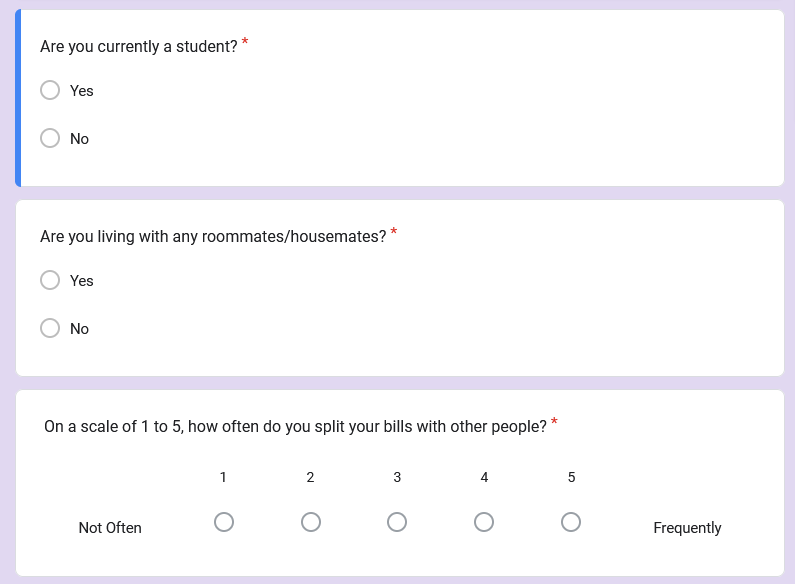
\includegraphics[width=1\linewidth]{survey_part_1.png}
    \caption{Part 1 of survey}
    \label{fig:pt1}
\end{figure}

\begin{figure}[H]
    \centering
    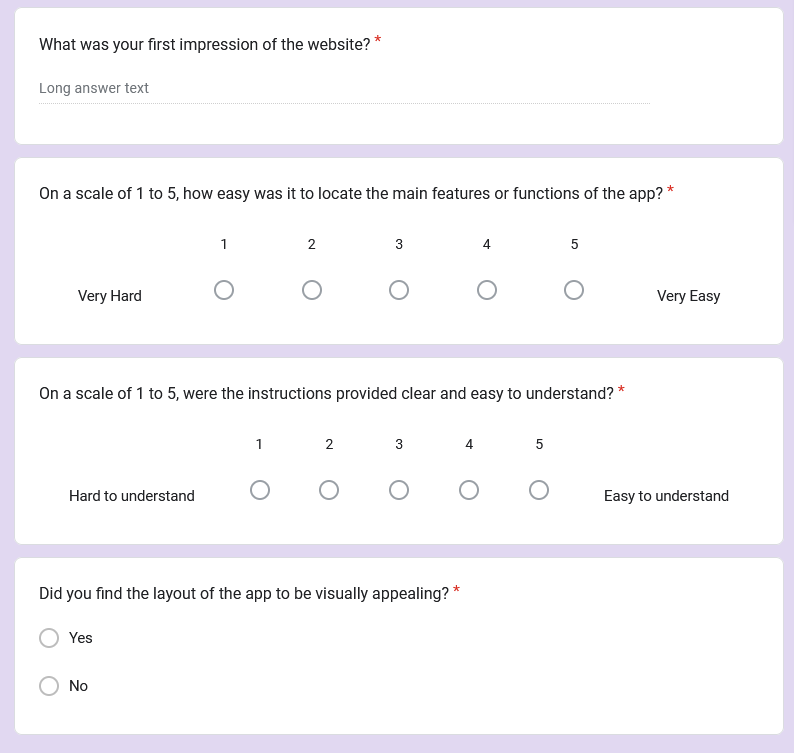
\includegraphics[width=1\linewidth]{survey_part_2.png}
    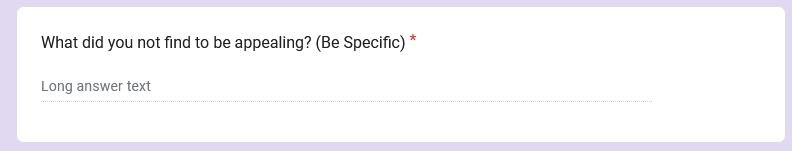
\includegraphics[width=1\linewidth]{survey_part_2_5.png}
    \caption{Part 2 of survey}
    \label{fig:pt2}
\end{figure}

\begin{figure}[H]
    \centering
    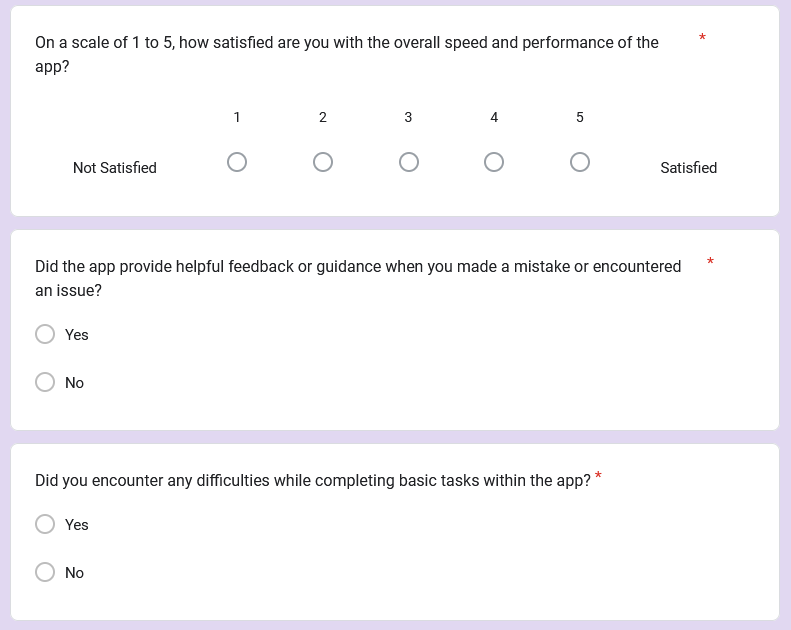
\includegraphics[width=1\linewidth]{survey_part_3.png}
    
\includegraphics[width=1\linewidth]{survey_part_3_5.png}
    \caption{Part 3 of survey}
    \label{fig:pt3}
\end{figure}

\begin{figure}[H]
    \centering
    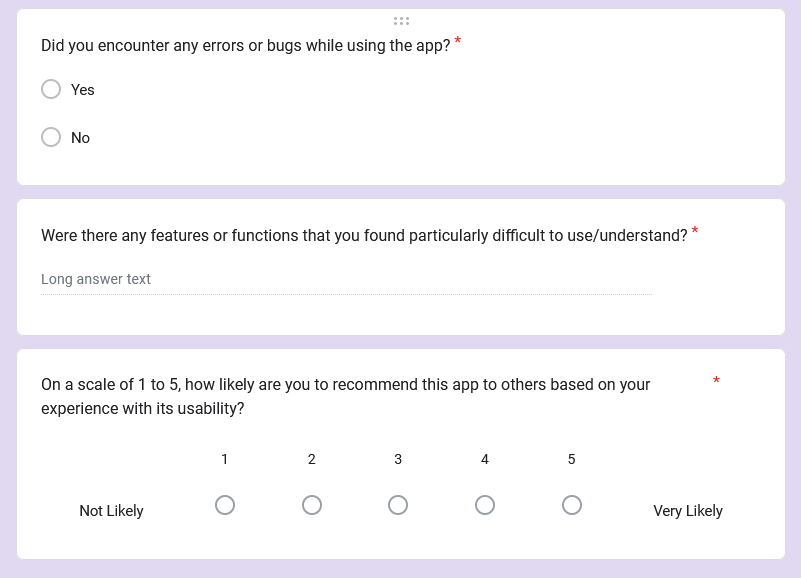
\includegraphics[width=1\linewidth]{survey_part_4.png}
    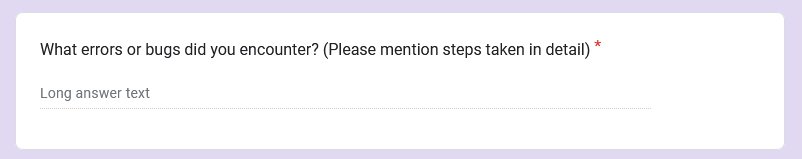
\includegraphics[width=1\linewidth]{survey_part_4_5.png}
    \caption{Part 4 of survey}
    \label{fig:pt4}
\end{figure}

% \begin{enumerate}
%     \item Do you have housemates?
%     \begin{enumerate}
%         \item Yes
%         \item No
%     \end{enumerate}
%     \item What operating system is run on your phone?
%     \begin{enumerate}
%         \item IOS
%         \item Android
%         \item Others
%     \end{enumerate}
%     \item What do you find frustrating about having housemates?
%     \item Which feature of the Housemates application do you find the most interesting/would use the most often?
%     \begin{enumerate}
%         \item Split bills
%         \item Delegate chores
%         \item Schedule events
%     \end{enumerate}
%     \item Did you find the Housemates application visually appealing and intuitive?
%     \begin{enumerate}
%         \item Yes
%         \item No
%     \end{enumerate}
%     \item Did you find the Housemates application easy to navigate?
%     \begin{enumerate}
%         \item Yes
%         \item No
%     \end{enumerate}
%     \item Did you find the features of the Housemate application easy to learn?
%     \begin{enumerate}
%         \item Yes
%         \item No
%     \end{enumerate}
%     \item Would you use the Housemates application in your regular life?
%     \begin{enumerate}
%         \item Yes
%         \item No
%     \end{enumerate}
% \end{enumerate}

% \wss{This is a section that would be appropriate for some projects.}

% \newpage{}
% \section*{Appendix --- Reflection}

% The information in this section will be used to evaluate the team members on the
% graduate attribute of Lifelong Learning.  Please answer the following questions:

\newpage{}
\subsection{Reflection}

% \wss{This section is not required for CAS 741}

The information in this section will be used to evaluate the team members on the
graduate attribute of Lifelong Learning.  Please answer the following questions:

\begin{enumerate}
  \item What knowledge and skills will the team collectively need to acquire to
  successfully complete the verification and validation of your project?
  Examples of possible knowledge and skills include dynamic testing knowledge,
  static testing knowledge, specific tool usage etc.  You should look to
  identify at least one item for each team member.
  \item For each of the knowledge areas and skills identified in the previous
  question, what are at least two approaches to acquiring the knowledge or
  mastering the skill?  Of the identified approaches, which will each team
  member pursue, and why did they make this choice?
\end{enumerate}

\subsubsection{Knowledge and Skills}
\begin{itemize}
    \item The team will need to learn how to use GitHub actions in order to be able to run automatic tests during CI/CD.
    \item The team needs to acquire dynamic testing knowledge in order to perform the tests in this VnV plan.
    \item The team needs to acquire usability testing knowledge in order to perform the tests in this VnV plan.
    \item The team needs to acquire static testing knowledge in order to perform the tests in this VnV plan.
    \item The team needs to acquire domain specific knowledge on React testing.
\end{itemize}

\subsubsection{Approaches}
\begin{itemize}
    \item GitHub Actions
    \begin{itemize}
        \item Watch/read online tutorials on GitHub Actions.
        \item Re-watch GitHub Actions tutorial for SFWRENG 4G06.
    \end{itemize}
    Fady Morcos: The approach chosen to acquire the GitHub skills/action I need to be successful here are to research, read and watch online tutorials on GitHub actions to reinforce my GitHub knowledge. Another thing I will do is re-watch the GitHub actions tutorial posted for the SFWRENG 4G06 course as this is should have reliable information summarized for all of my GitHub needs to be successful.
    \item Dynamic testing
    \begin{itemize}
        \item Research dynamic testing methods online.
        \item Look at SFWRENG 3S03: Software Testing notes on dynamic testing.
    \end{itemize}
    Rizwan Ahsan: The approach I will choose for learning dynamic testing is researching online to find good dynamic testing techniques. This will give me in-depth knowledge about dynamic testing techniques and allow me to find the best method to perform dynamic testing for our project.
    \item Static testing
    \begin{itemize}
        \item Research static testing methods online.
        \item Look at SFWRENG 3S03: Software Testing notes on static testing.
    \end{itemize}
    Fardeen Afsar: For static testing, I'll apply the techniques and methods introduced in SFWRENG 3S03, while focusing on usability in code and documentation review. This ensures early identification of defects and adherence to standards.  For static testing, I will also opt for a method focused on acquiring knowledge about static testing through online research.
    \item Usability testing
    \begin{itemize}
        \item Look at testing/research methods from SFWRENG 4HC3: Human Computer Interfaces.
        \item Research online methods for usability testing.
    \end{itemize}
    Justin Dang: The approach I chose for learning usability testing is taking methods used in SFWRENG 4HC3. This is because for 4HC3 we have had a focus on design for usability.
    \item Domain knowledge on React testing
    \begin{itemize}
        \item Watch React testing tutorials.
        \item Look at \href{https://jestjs.io/docs/tutorial-react}{React testing website}.
    \end{itemize}
    Harris Hamid: The approach I'm choosing to actually create test cases for our React web app will be to use jest, a JavaScript testing framework. I'll look at examples at how it is being used in actual production level code.
\end{itemize}

\end{document}